Cette expérience permet d'observer l'impact du niveau de reconstruction des flux quand l'opérateur de diffusion est couplé à un opérateur de diffusion et faisant émerger des dynamiques de couplage.
L'équation de diffusion est donc remplacée par l'équation de Nagumo (voir \ref{par:analyser_operateurs_nagumo}).
Des ondes progressives sont solution de cette équation, le schéma numérique donc doit être en mesure de suivre la dynamique du front d'onde.

\subsubsection{Résumé de l'expérience}
L'expérience à été réalisée dans des conditions similaires à l'expérience numérique \ref{par:contrib_imex}. 
C'est à dire :
\begin{itemize}
    \item[$\diamond$] Profil de l'onde propagative comme état initial.
    \item[$\diamond$] Domaine étendu avec conditions de Neumann aux limites pour limiter les effets de bord
\end{itemize}
L'unique différence majeur est le remplacement de la méthode Runge et Kutta ImEx par un schéma de séparation d'opérateur avec une méthode stabilisée explicite pour la diffusion (ROCK 2 \cite{AbdulleMedovikov2001}).
Ce choix découle, comme précédemment expliqué, de la nécessité d'éviter toute inversion de système linéaire lorsque les flux sont reconstruits à partir de reconstructions
fines.


\subsubsection{Résultats de l'expérience}
Les résultats de l'expérience sont donnés en figure \ref{fig:flux_reconstruction_nagumo}, selon le pas de temps les observation sont:
\begin{itemize}
    \item[$\diamond$] \textbf{Pas de temps "petits" - erreur spatiale dominante:} L'erreur se comporte pareillement au cas de la diffusion pure, plus les flux sont reconstruit finement, plus l'erreur augmente.
    \item[$\diamond$] \textbf{Pas de temps "grands" - erreur temporelle dominante:} L'erreur se comporte encore comme dans le cas de la diffusion pure, la méthode de reconstruction n'induite pas de variations sensibles de l'erreur.
    \item[$\diamond$] \textbf{Pas de temps 'intermédiaires" - erreur spatio-temporelle: } C'est l'observation la plus intéressante: plus les flux sont finement évalués, plus l'erreur chute brutalement. 
            Comme si \textit{la reconstruction fine des flux de diffusion prévenait un couplage des erreurs en temps et en espace}. Plus l'onde est raide, plus l'effondrement de l'erreur est marqué
            ce qui suggère que cette amélioration vient avant tout d'un meilleur suivi du front d'onde. Enfin, quand le pas de temps continue de diminuer, l'erreur remonte comme si 
            une sorte d'instabilité polluait la solution (voir figure AFAIRE). 
\end{itemize}
\begin{figure}[h!]
    \centering
    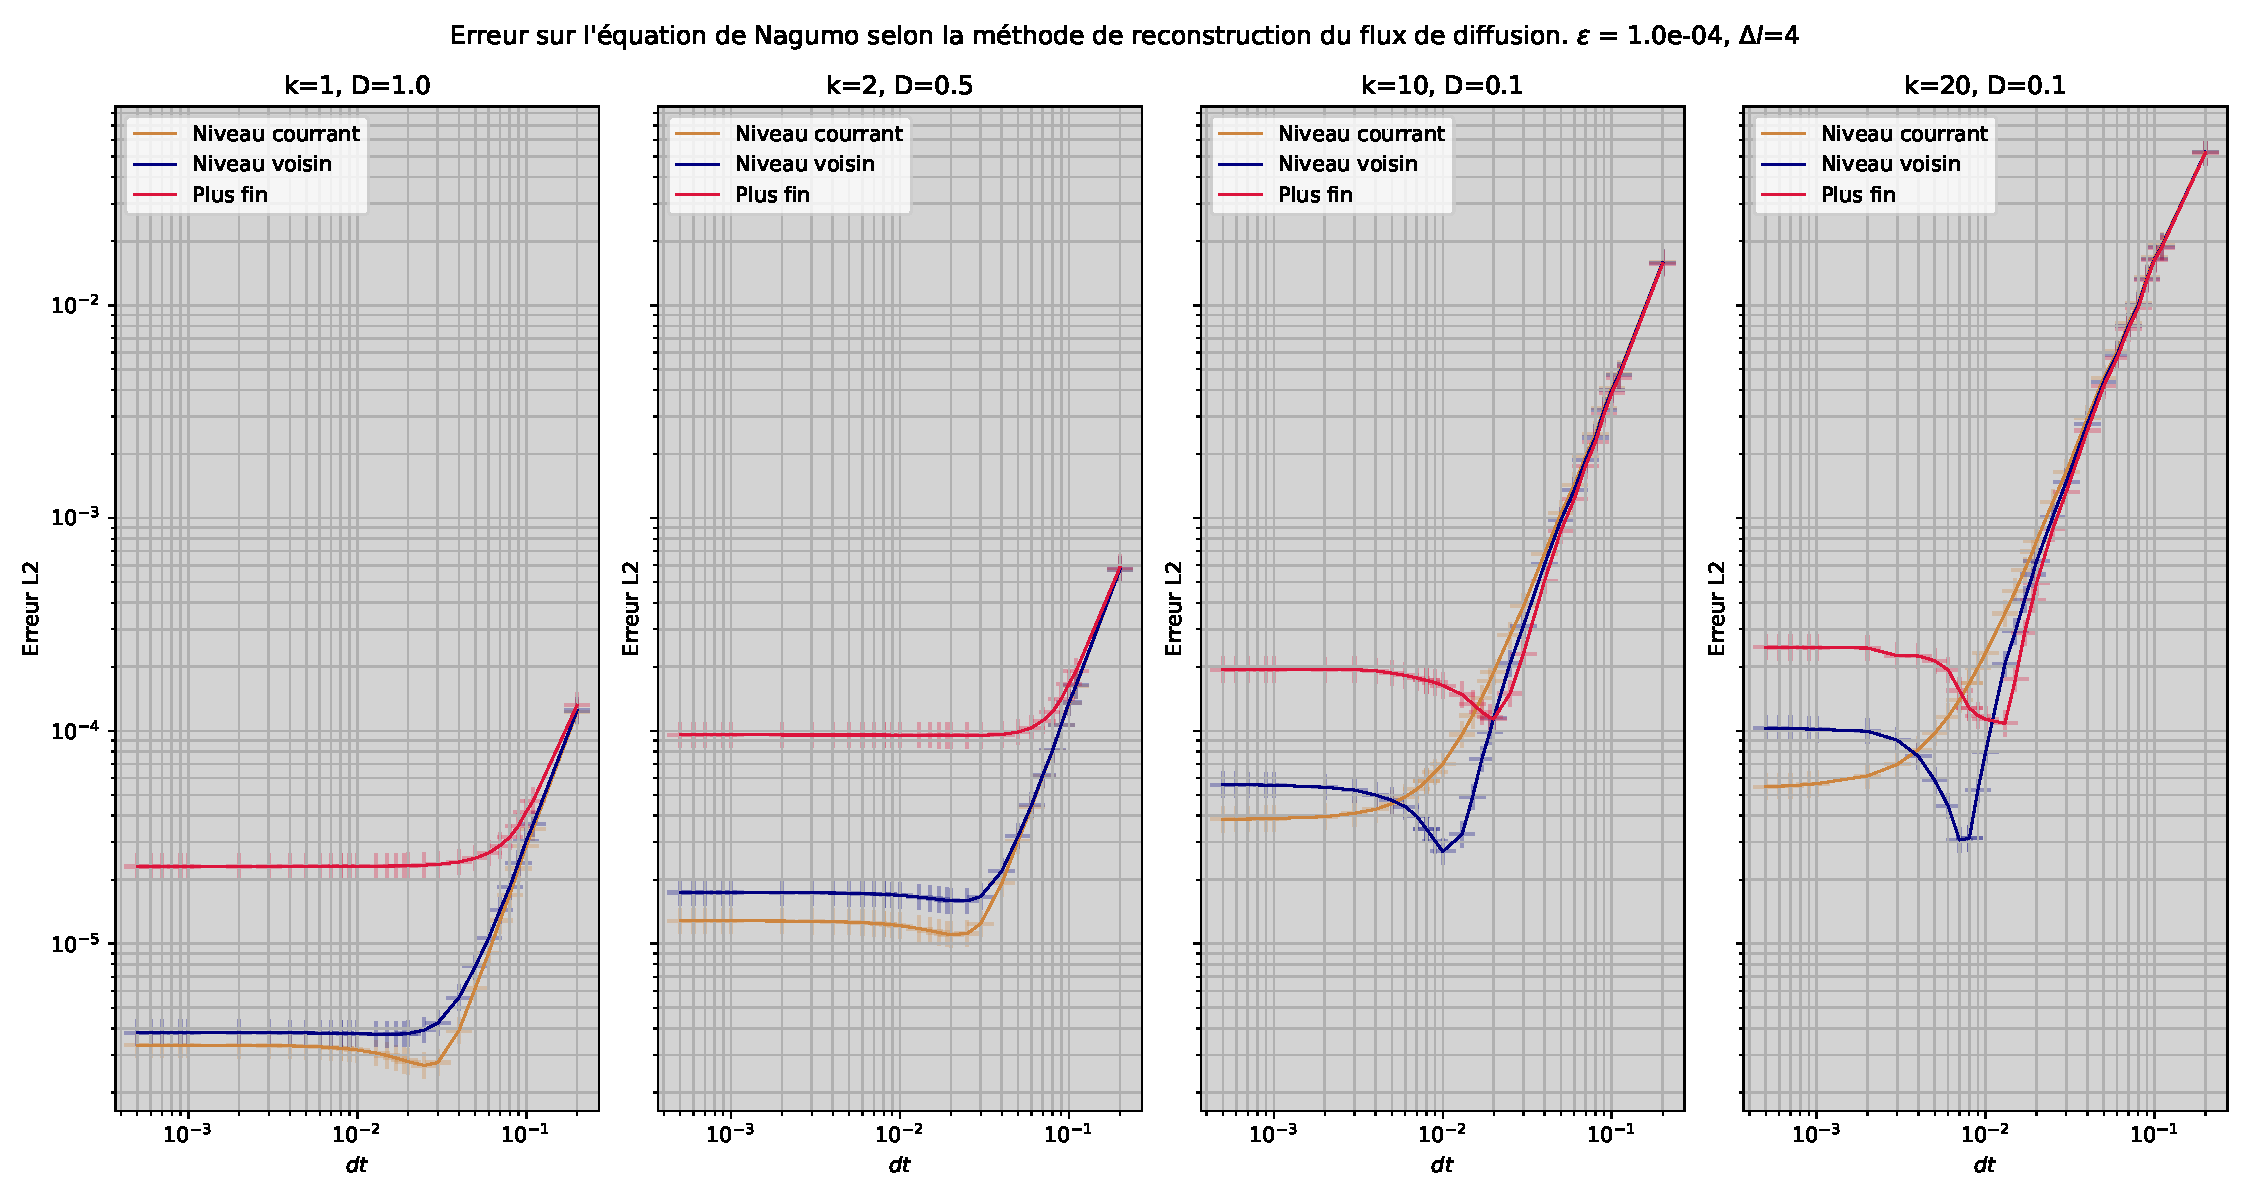
\includegraphics[width=\textwidth]{media/4_travail/3/flux_reconstruction_method_nagumo.pdf}
    \caption{Courbes de convergence de chaque méthode d'AMR pour différents paramètres de l'équation. Plus $k$ est élevé, plus le profil de l'onde est raide et plus la réaction domine. La célérité de l'onde est néanmoins identique pour chaque jeu de paramètres puisque le produit $kD$ reste constant d'une expérience à l'autre.}
    \label{fig:flux_reconstruction_nagumo}
\end{figure}